% SPDX-FileCopyrightText: 2023 SAP SE
%
% SPDX-License-Identifier: Apache-2.0
%
% This file is part of FEDEM - https://openfedem.org

%%%%%%%%%%%%%%%%%%%%%%%%%%%%%%%%%%%%%%%%%%%%%%%%%%%%%%%%%%%%%%%%%%%%%%%%%%%%%%%%
%
% FEDEM Theory Guide.
%
%%%%%%%%%%%%%%%%%%%%%%%%%%%%%%%%%%%%%%%%%%%%%%%%%%%%%%%%%%%%%%%%%%%%%%%%%%%%%%%%

\section{Joint Friction}

Friction is calculated from forces, moments, and relative velocity in a joint.
The friction properties consist of viscous friction, Coulomb dry friction,
modified Stribeck friction, and friction force caused by prestressed components.
The Stribeck friction yields a continuous description of the friction from
static to sliding movement.

Forces and moments in the joint give an equivalent load, which is the basis for
computing the acting friction force in the joint.
The equivalent load for the various joint types is given in the
Sections~\ref{subs:FricRevJoint}--\ref{subs:FricCamJoint} below.


\subsection{Viscous friction}

Viscous friction can act between any two supernodes or on any joint variable.
The damper force or torque is equal to the damper's viscous coefficient
multiplied by the damper velocity.
%
\begin{equation}
F_{\textit{viscous}} \;=\; c\: V
\end{equation}
%
where $c$ is the damper coefficient.


\subsection{Coulomb friction}

\begin{figure}[b]
\center{
\setlength{\unitlength}{1.2mm}
\begin{picture}(70,40)(-20,-18)
% Axis system
\thinlines
\put(-20,  0){\vector(1,0){60}}
\put(  0,-18){\vector(0,1){38}}
\put( -5,  7){\rotatebox{90}{\textsl{Friction}}}
\put( -1, 21){$F$}
\put( 20, -5){\textsl{Velocity}}
\put( 42, -1){$V$}
%The actual damping function
\thicklines
\put(-20,-10){\line(1,0){20}}
\put(  0,-10){\line(0,1){20}}
\put(  0, 10){\line(1,0){30}}
\put( 32,  9){$F_{\textit{Coulomb}}$}
\end{picture}
}
\caption{Coulomb friction}
\label{figFRIC:Coulomb}
\end{figure}

In classical Coulomb friction models, there is a constant friction force
opposing the motion when the velocity is non-zero. In the case of zero velocity,
the friction opposes all motions as long as the force is smaller in magnitude
than the friction force (see Figure~\ref{figFRIC:Coulomb})
%
\begin{equation}
F_{\textit{Coulomb}} \;=\; \mu_{\textit{Coulomb}}\: F_e\: \text{sgn}(V)
\end{equation}
%
where
%
\begin{namelist}{$\mu_{\textit{Coulomb}}$}
\item[$F_{\textit{Coulomb}}$]   : Coulomb friction force
\item[$\mu_{\textit{Coulomb}}$] : Coefficient of friction
\item[$F_e$]                    : Equivalent normal load
\item[$V$]                      : Velocity
\item[$\text{sgn}(V)$]          : The direction of movement ($\pm 1$)
\end{namelist}

Reduction gears and bearing set-ups are often prestressed to avoid backlash.
This prestress produces friction even when the external load is zero.
This friction component, which is added to the Coulomb friction term.
is defined as (see Figure~\ref{figFric:Prestress}):
%
\begin{equation}
F_{\textit{prestress}} \;=\; F_0\: \text{sgn}(V)
\end{equation}
%
where $F_0$ is the friction force or torque caused by prestressed components
or other constant friction effects.

\begin{figure}[b]
\center{
\setlength{\unitlength}{1.1mm}
%===================== First picture =========================
\begin{picture}(50,45)(-20,-20)
% Axis system
\thinlines
\put(-20,  0){\vector(1,0){45}}
\put(  0,-20){\vector(0,1){40}}
\put( -5, 21){\textsl{Friction}}
\put( 10, -5){\textsl{Velocity}}
\put( 27, -1){$V$}
%The actual friction function
\thicklines
\qbezier[30](-20,-12.5)(-10,-12.5)( 0,-12.5)
\qbezier[30](-20,-10  )(-10,-10  )( 0,-10  )
\qbezier[30](  0, 10  )( 10, 10  )(20, 10  )
\qbezier[30](  0, 12.5)( 10, 12.5)(20, 12.5)
\put(-20,-7.5){\line(1,0){20}}
\put(  0,-7.5){\line(0,1){15}}
\put(  0, 7.5){\line(1,0){20}}
\end{picture}
\hfill
%================== Second picture ==========================
\begin{picture}(50,45)(-20,-20)
% Axis system
\thinlines
\put(-20,  0){\vector(1,0){45}}
\put(  0,-20){\vector(0,1){40}}
\put( -5, 21){\textsl{Friction}}
\put( 10, -5){\textsl{Normal load}}
\put( 27, -1){$F_e$}
\put( -5,  4){$F_0$}
\put(  1, -6){$-F_0$}
%The actual friction function
\thicklines
\qbezier(-20,-9)(-10,-7)( 0,-5)
\qbezier(  0, 5)( 10, 7)(20, 9)
\put(0,-5){\line(0,1){10}}
\end{picture}
}
\caption{Friction caused by prestressed components}
\label{figFric:Prestress}
\end{figure}


\subsection{Modified Stribeck friction}

\begin{figure}[b]
\center{
\setlength{\unitlength}{1.3mm}
\begin{picture}(85,65)(-30,-30)
% Axis system
\thinlines
\put(-30,  0){\vector(1,0){80}}
\put(  0,-30){\vector(0,1){60}}
\put( -5, 32){\textsl{Friction}}
\put( 52, -1){$V$}
%The actual friction function
\thicklines
\qbezier( 0, 20  )(  6, 20)(  8, 16.5)
\qbezier( 8, 16.5)( 10, 13)( 22, 13  )
\qbezier( 0,-20  )( -6,-20)( -8,-16.5)
\qbezier(-8,-16.5)(-10,-13)(-22,-13  )
\put(0, 13){\line( 1,0){38}}
\put(0,-13){\line(-1,0){25}}
\put(0,-20){\line( 0,1){40}}
%
%Equations
\thinlines
\qbezier[30]( 0,20)( 9   ,20  )(18  ,20  )
\put(20  ,19){$F_{\textit{Static}}= (1+S)F_{\textit{Coulomb}}$}
\qbezier[8] (39,13)(41.75,13  )(44.5,13  )
\put(45.5,12){$F_{\textit{Coulomb}}$}
\qbezier[26]( 8,-1)( 8   ,7.75)( 8  ,16.5)
\put( 6.5,-4){$V_{\textit{slip}}$}
%
%Arrows
\thicklines
\put( 0,  6){\vector( 0, 1){3}}
\put( 0,  6){\vector( 0,-1){3}}
\put( 0, 17){\vector( 0, 1){1}}
\put(31, 13){\vector( 1, 0){3}}
\put(31, 13){\vector(-1, 0){3}}
\put( 6, 13){\vector(-1, 0){1}}
\put( 0, -6){\vector( 0, 1){3}}
\put( 0, -6){\vector( 0,-1){3}}
\put( 0,-17){\vector( 0,-1){1}}
\put(-6,-13){\vector( 1, 0){1}}
\put( 7, 18){\vector( 1,-1){1}}
\put(-7,-18){\vector(-1, 1){1}}
\end{picture}
}
\caption{Modified Stribeck friction including hysteresis}
\label{figFric:ModStribeck}
\end{figure}

Modified Stribeck friction defines friction as a constant at extremely low
velocities, then making a smooth transition from higher static friction to the
lower kinetic, or kinetic plus viscous, friction.
A model using modified Stribeck friction predicts a steady motion at extremely
low velocities, instability through a range of velocities, and stable motion
above a certain threshold velocity.

Experiments have verified that after the stiction force has been surmounted,
the friction decreases exponentially reaching approximately 60\% of the
breakaway force. These bends occur at velocities close to zero.
Detailed experiments carried out in industrial manipulators and reduction gears
have confirmed this negative velocity dependence at low velocity.
The hysteresis effect is also added into the Stribeck friction.
It has been observed that the friction curve is not single-valued.
There is a static friction force that is higher than the kinetic friction,
and the friction does not return to the higher static value when the sliding
velocity decreases.
This means that the friction remains at the low Coulomb friction value until
the velocity has changed sign or is zero (see Figure~\ref{figFric:ModStribeck}):
%
\begin{equation}
F_{\textit{Stribeck}} \;=\; F_{\textit{Coulomb}}
(1 + S e^{-(\frac{V}{V_{\textit{slip}}})^2})\: \text{sgn}(V)
\end{equation}
%
where
%
\begin{namelist}{$F_{\textit{Coulomb}}$}
\item[$F_{\textit{Stribeck}}$] : Stick-slip friction as a function of velocity
\item[$F_{\textit{Coulomb}}$]  : Coulomb friction including friction from
                                 prestressed \mbox{\hskip4pt}~components
\item[$S$] : Magnitude of Stribeck effect (stick-slip factor):
\[ S = \frac{F_{\textit{static}}-F_{\textit{Coulomb}}}{F_{\textit{Coulomb}}} \]
\item[$V_{\textit{slip}}$]     : Critical velocity for Stribeck effect
\item[$\text{sgn}(V)$]         : The direction of movement ($\pm 1$)
\end{namelist}


\subsection{Total friction}

The total friction model is a function resulting from the combination of the
three components described above:
%
\begin{equation}
F_{\textit{total}} \;=\; F_{\textit{viscous}} +
\left[ F_0 + \mu_{\textit{Coulomb}} \: F_e
\left( 1 + S e^{-(\frac{V}{V_{\textit{slip}}})^2}
\right)\right]\: \text{sgn}(V)
\end{equation}


\subsection{Equivalent load in revolute joint}
\label{subs:FricRevJoint}

Friction in revolute joints depends on bearing design and joint loads.
The revolute joint transmits the forces $F_x$, $F_y$, and $F_z$ and the bending
moments $M_x$ and $M_y$.
All these forces and moments are carried by the joint bearings.
The first step is to calculate the axial and radial bearing load based on these
joint forces and moments.

\begin{figure}[b]
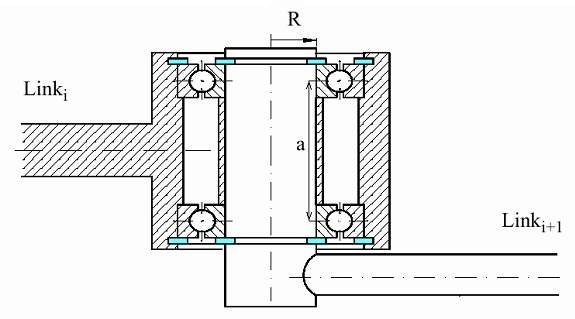
\includegraphics[width=\textwidth]{Figures/FricRevJoint.png}
\caption{Revolute joint}
\label{figFric:RevJoint}
\end{figure}

The revolute joint can be designed and modeled in many ways.
In some cases the joint has only one bearing.
The bending capacity is then calculated by the bearing constant $a$.
This is a standard constant given in bearing catalogs.
If the joint has two bearings as shown in Figure~\ref{figFric:RevJoint},
the joint can also be modeled by using two separate revolute joints,
one at each bearing.
The next step is to calculate the equivalent bearing load as a function of axial
and radial bearing load and bearing geometry. Different types of bearings are
designed to carry either radial or axial load or a combination of these loads.
The equivalent load is then calculated as follows:
%
\begin{eqnarray}
\text{Bearing 1:}\hskip7pt
F_{rx1} &=& \frac{F_x}{2} - \frac{M_y}{a} \nonumber\\
F_{ry1} &=& \frac{F_y}{2} - \frac{M_x}{a} \nonumber\\
F_{r1}  &=& \sqrt{F_{rx1}^2 + F_{ry1}^2} \\[3mm]
%
\text{Bearing 2:}\hskip7pt
F_{rx2} &=& \frac{F_x}{2} + \frac{M_y}{a} \nonumber\\
F_{ry2} &=& \frac{F_y}{2} + \frac{M_x}{a} \nonumber\\
F_{r2}  &=& \sqrt{F_{rx2}^2 + F_{ry2}^2} \\[3mm]
%
\text{Radial bearing load:}\hskip15pt
F_r &=& F_{r1} + F_{r2} \\[1mm]
\text{Axial bearing load:}\hskip15pt
F_a &=& F_z \\[2mm]
%
\text{Equivalent bearing load:}\hskip15pt
\label{eq:BearingLoad}
F_e &=& F_r + F_a Y
\end{eqnarray}
%
where $Y$ is a constant depending on bearing type and geometry, and is
given in the bearing catalogs.
The friction force is calculated as a function of the equivalent bearing load
and the angular velocity. The friction torque in the joint is calculated by
multiplying the friction force by the bearing radius $R$.

A simplified friction representation in revolute joints, where the effects of
the bending moments and the axial load are ignored can also be used.
The coefficients $a$ and $Y$ are then not needed and the equivalent normal
load given by \eqnref{eq:BearingLoad}, reduces to
%
\begin{equation}
\label{eq:RevJointLoad}
F_e \;=\; \sqrt{F_x^2 + F_y^2}
\end{equation}


\subsection{Equivalent load in ball and free joints}

Ball and free joints can both be assigned friction properties to one of its
three rotational DOFs.
The equivalent normal load is then given by \eqnref{eq:RevJointLoad}, where the
indices $x$ and $y$ now represent the two local joint directions that are
orthogonal to the local axis of the chosen friction DOF.
The actual friction torque is then calculated in the same way as for a revolute
joint, based on a specified ball radius $R$ and the angular velocity in the
chosen friction DOF.

For free joints, friction can also be assigned to a translational DOF instead
of a rotational DOF.
The equivalent normal load is then 
%
\begin{equation}
\label{eq:FreeJointLoad}
F_e \;=\; \left\{\eqalign{
F_{e1} = \sqrt{F_y^2 + F_z^2} & \hskip5mm\text{for friction in the Tx DOF} \cr
F_{e2} = \sqrt{F_z^2 + F_x^2} & \hskip5mm\text{for friction in the Ty DOF} \cr
F_{e3} = \sqrt{F_x^2 + F_y^2} & \hskip5mm\text{for friction in the Tz DOF}
}\right.
\end{equation}
%
where $F_x$, $F_y$ and $F_z$ are the joint forces in its local directions.
The actual friction force is then calculated as a function of $F_e$ and
the linear velocity in the chosen friction direction.

\subsection{Equivalent load in prismatic joint}

The friction in a prismatic joint depends on forces normal to the sliding axis
($z$-axis) and forces caused by torque around the $z$-axis.
The joint rotation around the $z$-axis is fixed.
This is usually accomplished by means of a sliding key or similar mechanism
(see Figure~\ref{figFRIC:Prism}).

The friction coefficient in the locking device can in some cases be much higher
than in the linear guidance. This linear bearing is often made of low-friction
rolling elements. Forces in the locking device and normal load in the guidance
are therefore separated and can be weighted by the factor $Y$.
%
\begin{figure}[b]
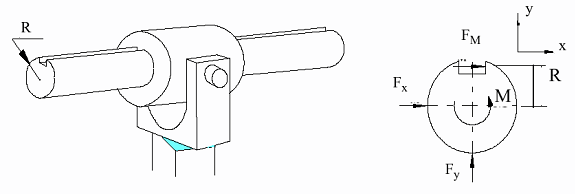
\includegraphics[width=\textwidth]{Figures/FricPriJoint.png}
\caption{Prismatic joint}
\label{figFRIC:Prism}
\end{figure}
%
\begin{eqnarray}
\text{Normal Force:} && F_N \;=\; \sqrt{F_y^2 + (F_x - \frac{M_z}{R})^2} \\
\text{Force in locking device:} && F_M \;=\; \frac{M_z}{R}
\end{eqnarray}
%
Here (see Figure~\ref{figFRIC:Prism}),
$F_y$ and $F_x$ are joint forces in the $y$ and $z$ direction,
$M_z$ is the torque around the sliding $z$-axis, and
$R$ is the radius or distance to the locking device.
The equivalent load is then given by
%
\begin{equation}
\label{eq:PrismLoad}
F_e \;=\; F_N + F_M Y
\end{equation}

A simplified friction representation in prismatic joints, where the effects of
the locking device is ignored can also be used.
The coefficients $R$ and $Y$ are then not needed and the equivalent normal
load, \eqnref{eq:PrismLoad}, reduces to $F_{e3}$ of \eqnref{eq:FreeJointLoad}.

The actual friction force in the prismatic joint is calculated as a function
of the equivalent normal load and the linear velocity of the slider DOF.


\subsection{Equivalent load in cam joint}
\label{subs:FricCamJoint}

The equivalent load in a cam joint is the force between the cam and the follower
in the normal ($x$) direction.
No effect from any translation in the $y$-direction is accounted for.
The equivalent force $F_e$ is thus equal to the force of the contact spring
in the $x$-direction, and the actual friction force is calculated similarly
as for the prismatic joint.
